% 10:57 04/04/2023
\chapter{Methodology}
% Describe the way you went about your project.
% Was your approach to the problem valid?
% You need to discuss both your software development
% methodology and your research methodology.

This chapter will be discussing the methodology,
That I used whilst developing my project
along with the research that helped guide it.
The primary objective of my research was to identify components,
that would allow my platform to detect malware based on its behaviour.
These components include Sandboxie and Process Monitor.

Git played an important role during the development of the project.
It is also used to host my promotional page,
and it uses GitHub Pages to automatically deploy it.
I also used GitHub Actions to run a suite of tests on the
API endpoints when code was pushed to the repository.
To manage tasks and time effectively, I used a Kanban board on GitHub
and adopted an agile-style methodology to ensure
progress with changing requirements.
And I used Docker to create a reproducible environment,
to avoid having to install and set up dependencies for different machines.
The server will be hosted on the Microsoft Azure Cloud.

\section{Determining Requirements}
I recognised that most anti-malware solutions targeting consumers
come with a GUI application for performing scans.
I wanted to do the same, which is why there is a GUI application.

There would be a server component and a database to persist data for the server.
After some thought, I decided against performing scanning on the server.
Instead, I opted to have the scanning done on separate analysis workers.
This would isolate any potential malware from compromising the server and
allows for multiple scans at the same time.

For communication between the clients and the server, I chose to use RESTful APIs.
I chose this because it is now the de facto standard for web applications and is quite simple.

I also included a dashboard to provide a user-friendly interface for administrators,
enabling them to perform actions on the platform as a whole without
having to do it through a tedious command-line interface.

\section{Research}
When I figured out what I wanted to do my project on
(that being malware detection),
I conducted research on the various technologies that I could use.
My initial focus was on tools that would enable me
to log the system calls on Windows.
Although I initially considered creating the logging software myself,
I quickly realised that this would be too time-consuming,
preventing me from creating a fully-featured platform in the time given.

My research led me to discover "Process Monitor" \cite{procmon},
a software by Microsoft that can be used to log system calls.
I also explored open-source software that
I could use to do static analysis.
I was originally going to do only dynamic analysis
but there is always the potential of it not detecting malware,
and there are already definitions of known malware on the internet.
I discovered ClamAV and opted for its Windows-optimised version, ClamWin.
This software periodically downloads definition signatures
of known malware in the wild.

One of the biggest challenges I faced was finding a way to
run potentially malicious software safely
in an isolated environment without harming the
computer running the software.
After exploring the potential options,
I settled for Sandboxie. \cite{sandboxie}
I initially considered running the software on a virtual machine,
Sandboxie proved to be a more efficient option.
This software works by hooking the operating-system, system calls.
Sandboxie keeps track of what resources a running
process has permission to access.
It also has the ability to hide files from the running process.

\subsection{Collecting System Calls}
After choosing Process Monitor as my tool to collect system calls,
I needed to find a way to integrate it into my project.
While most people use Process Monitor's user interface
to click buttons and navigate using its interface,
I needed a method of using it automatically
without manually directing it each time.
Thankfully, I discovered that Process Monitor supports some command-line
options which can be viewed by typing "\textbf{procmon.exe /?}".
This allowed me to start and stop Process Monitor as needed.

Through experimentation, I found a way to start
Process Monitor from my Racket program.
I would then spawn the program I was observing and record its behaviour.
Once it was finished, I would then shut down Process Monitor
and convert the data it collected into a usable CSV format.
To start Process Monitor with a minimized window,
I used the command
"\textbf{procmon.exe /Minimized /BackingFile output-location.pml}",
which produces a PML file. After the monitored process had finished,
I passed the \textbf{/Terminate} parameter to Process Monitor to stop monitoring.

I struggled to find much documentation on the PML format,
I then found that Process Monitor had a parameter to convert it to CSV format.
By using "\textbf{/OpenLog output-location.pml /SaveAs csv-location.csv}",
I could output a plain-text file with each system call on a new line.
One final problem was that Process Monitor didn't have the ability
to filter out processes I wasn't interested in,
so I made a Python script that filters out everything that
isn't the process and it's children.

\subsection{Client Installer}
For users to be able to install the client on their computer(s),
I researched tools that could generate a Windows installer.
I came across a tool called \textbf{iexpress.exe},
which is conveniently included in Windows.

\textbf{iexpress.exe} is primarily used through its GUI,
I discovered that it can accept a parameter through the command-line,
a SED file (\textbf{client/caladium.sed})
containing instructions for iexpress to build an installer.

Before creating the installer,
I archived all the files generated by PyInstaller into a tarball (tar.gz)
and included a script with the installer that
extracts the archive into the \texttt{Program Files} directory on Windows.
I also have it so it creates a shortcut in the startup directory,
so it starts on system boot.

\section{Development}
For version control, I used Git and hosted the repository on GitHub.
I added a \texttt{.gitignore} to prevent temporary files
and build outputs from being pushed to the repository.
Initially, I divided the project into
three parts: the client, server, and sandbox,
to maintain organisation. I then created a \textbf{src} subdirectory
for each sub-project, containing only the core code for that project.
For instance, the server subproject has a \textbf{tests} directory
containing test code that is not part of the core code.
Like the server, I moved the core code of the client to the
\textbf{src} subdirectory, leaving
the installer code in its original directory.

I worked mainly on Windows, but I occasionally switched
between different operating systems. To avoid working on
a stale version, I regularly committed changes to the
GitHub repository and pulled the latest version of the
repository to the current workstation. For text editing,
I used Visual Studio Code, which provides text suggestions,
and I occasionally used VIM to edit smaller scripts and files,
especially when working on Racket code.
I used Overleaf to write the dissertation and pushed the changes to the
\texttt{dissertation} directory in the GitHub repository.

Finding time to work on the project was challenging,
as I had other modules besides the dissertation.
I mostly worked on the project during weekends, and whenever
I thought of a new feature, I would then add it to the Kanban board.
During development, I spent a considerable amount of time thinking
about possible solutions to problems. For example,
to avoid embedding ugly HTML in my dashboard single application's JavaScript,
I created a library called \textbf{pantothenic.js} that can convert 
string-based Lisp expressions into DOM objects
(you'll see more about this in the design chapter).

\subsection{Weekly Progress Reports}
Every week during the 2 semesters, I exchanged my progress report,
with my supervisor during our weekly meeting over Microsoft Teams.

Below you will find each week's report and a description of what I did,
this would sometimes be research and/or development.

\textbf{16th - 22th of October} \\
I worked on the \texttt{DirChangeListener} class for the client,
which is used to listen for changes in directories.

This will be used to detect new files added to the downloads directory.
I researched methods of implementing the sandbox analysis,
and have a basic prototype of it working.

\textbf{23rd - 29th of October} \\
I found out that the system call logger was collecting too many system calls.
So I needed to filter out the ones I'm not interested in.
I made a filtering program in Python to do this.

I also refactored the analysis code to make it cleaner.

\textbf{30th of October - 12th of November} \\
I started using the Kanban board on GitHub to keep track of tasks.
I added code to the sandbox analysis service, so you can now connect to it over TCP,
and pass in a JSON message object containing the instructions you want it to execute.

\textbf{13th - 19th of November} \\
This week I was working on the dashboard, and I added a stylesheet called Milligram,
I enabled CORS, so I could now fetch data from the server without getting an error message.

\textbf{20th - 26th of November} \\
I worked on setting up Docker and a server on Azure.
Now I can run the server in a container, and it downloads all the dependencies I require.

\textbf{27th of November - 3rd of December} \\
I worked on setting up a page for adding workers in the dashboard application.
I also added backend logic for logging in users.

\textbf{4th - 10th of December} \\
I added code that can begin a scanning task on the server,
and added RESTful APIs for performing actions on this code.

\textbf{11th of December - 28th of January} \\
During these four weeks, I have:
\begin{itemize}
    \item Added CouchDB to store records rather than storing them in memory.
    \item Added a window to the client to display the scanning progress.
    \item Made a test suite to test the server API endpoints.
    \item Added code to display pie charts and bar charts.
    \item Added a preferences menu to the dashboard,
    so admins can change their passwords.
\end{itemize}

\textbf{29th of January - 4th of February} \\
I have restructured the architecture of the client,
requiring the client to be provisioned with the server, on the first startup.
All requests from the client to the server, 
are now authenticated, and you can't do anything without being first provisioned.
Files dropped into the downloads directory, now trigger a notification,
asking the user if they want the files to be scanned.
And I fixed some broken endpoints for deleting records, which the tests caught.

\textbf{5th - 11th of February} \\
During this week, I added a GitHub Action to automatically run the test suite,
when new code is pushed to the repository.
Fixed some problems in the client and server,
and fixed the problem in the client that was causing the scan to fail.
Clients can now auto-provision without requiring an admin to do it for them.

\textbf{12th - 18th of February} \\
This week, I successfully found a way to bundle the client code using PyInstaller.
I also created an installer using the \texttt{iexpress.exe} tool found in Windows
that creates a shortcut on installation.
Added commentary to some of the code,
I've restructured some of the code in the client to make it more smooth.

\textbf{19th - 25th of February} \\
I added a new preferences page to the client,
so users could update the current scanning directory.
Added a button to unprovision the client, I also added an icon to the executable,
fixed the bar chart rendering bug in the dashboard.

\textbf{26th of February - 4th of March} \\
I implemented the uninstall functionality in the preferences menu, in the client.
I added the code to do the static analysis with ClamAV.
I created a promotional page in the \texttt{/docs} directory
that will automatically be deployed to GitHub Pages, upon pushing to the repository.
Removing all threading code from the client, making it all asynchronous.

\textbf{5th - 11th of March} \\
I worked on the promotional page, adding a download button to
download the latest version of Caladium.
When malware is detected the user is now
prompted to quarantine the malicious files.
I have now made a \textbf{v0.1} release of the software on GitHub
along with a new feature, showing the current scanning directory on the main page.

\textbf{12th - 18th of March} \\
I made the scanning less likely to fail, by adding code to detect exceptions.
Added a new button on the admin dashboard to disable dynamic scanning.

\textbf{19th - 25th of March} \\
I fixed the remaining bugs in the scanning process,
finished the README and created a screencast.

Added a GPT-3.5 chatbot to the promotional page,
the chatbot allows new users to ask questions about the platform.

Fixed the pie chart rendering for the clean-malware ratio in the dashboard.
Found an XSS security vulnerability that has now been fixed.
And set a timeout for infinitely running scans,
to be killed after a minute in the dynamic analysis.

Added a 6th \textbf{v0.1.2} release of the client to GitHub.

\textbf{26th March - 15th April}
% 

\section{Agile Methodology}
I decided on an agile-style methodology because
I didn't have a complete understanding of everything I needed to do.

I didn't create a specification document in the beginning,
because I hadn't fully decided on the components to use,
for example, I didn't choose my database until December,
but I proceeded with working on the other components.

One of the benefits of using Agile is that it provides developers
with the ability to adapt to changing requirements,
which allows for more flexibility during the development process.
After running a suite of tests on the code,
it can be deployed to production if it passes all of them.

In order to manage the tasks required for the project,
I decided to break them down and create a Kanban board.
Initially, I was considering using Jira, but I later found out that
GitHub supported the Kanban board,
which was much more convenient because it was integrated with GitHub.
Throughout the development process,
I continuously identified the tasks that needed to be completed.

The Kanban board had three columns: "Todo", "In Progress", and "Done".
When I thought of a task that needed to be done,
I placed it in the "Todo" column.
When a task was in progress, I moved it to the "In Progress" column.
Once I finished working on a task, I then moved it to the "Done" column.
Appendix \ref{table:kanbanBoard} contains a list of
all the tasks I had on my Kanban board,
every one of them are now in the "Done" column.

Below you can find a screenshot of the Kanban board I used.
\begin{figure}[h!]
    \centering
    \label{image:kanbanBoardScreenshot}
    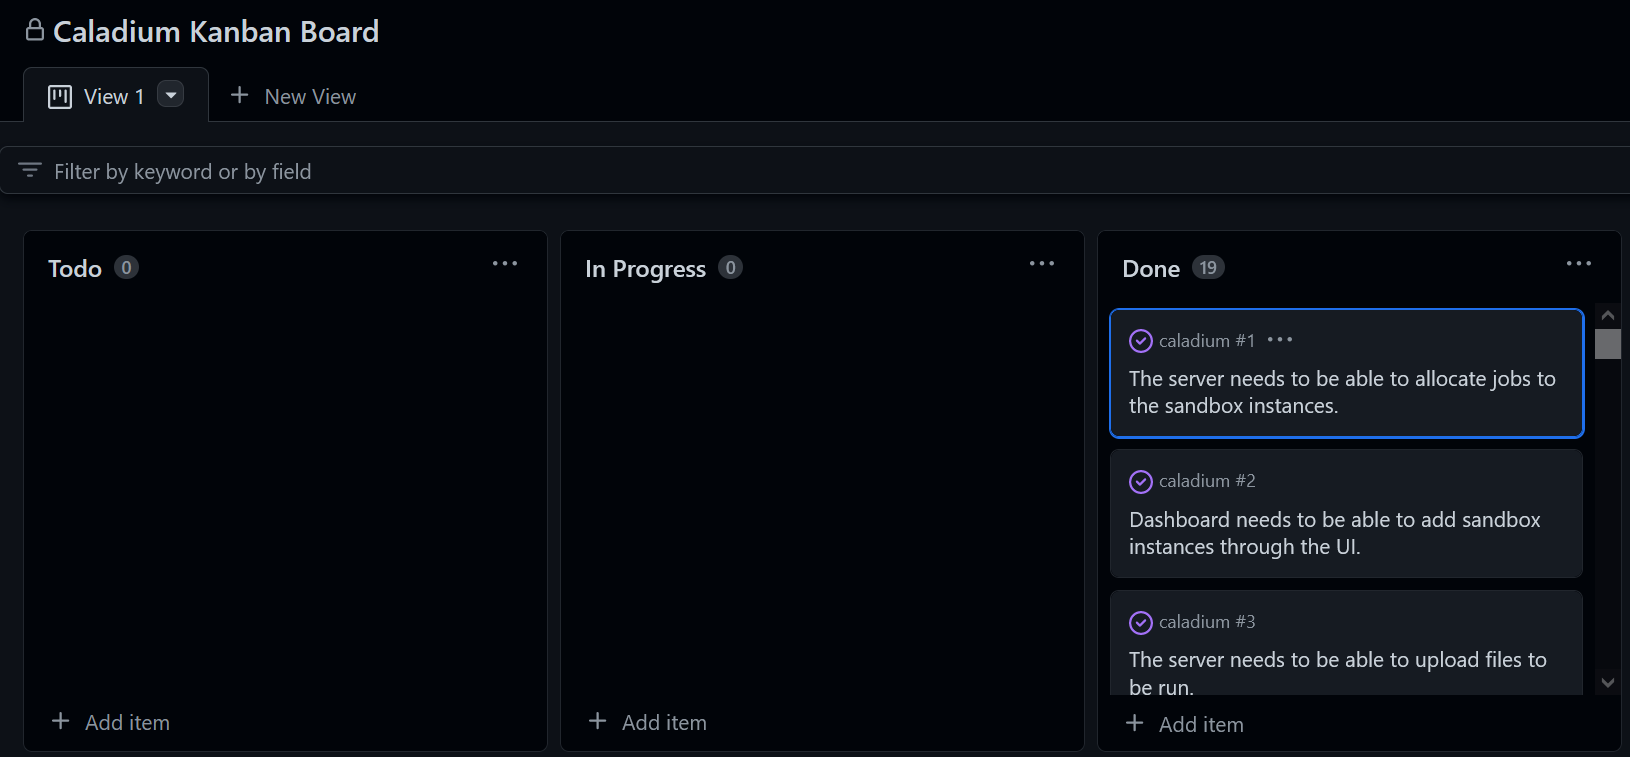
\includegraphics[width=0.95\textwidth]{images/screenshots/kanban_board}
    \caption{Kanban Board Screenshot}
\end{figure}

Every couple of weeks in the 2nd semester,
I created GitHub releases for the client.
These releases included the installer.
I followed the principles of semantic versioning,
where the version numbers are formatted as major.minor.patch.
By the end of the development,
I had reached version \texttt{v0.1.2}, which was the 6th release.

% What about validation and testing?
\section{Software Testing}
I used a test-driven approach (TDD) to develop the server endpoints.
I used the "unittest" Python library to write unit tests for the server endpoints.

I used the tests as a specification for the server endpoints.
If the tests failed, it indicated I wasn't implementing the endpoints correctly.
I could run the tests and it would verify if I had broken any of the endpoints.

The test files are prefixed with \textbf{test\_},
these test the \textbf{clients}, \textbf{patterns},
\textbf{tasks} and \textbf{workers} endpoints,
the endpoints are very similar, so I have each test file
inherit code from the \texttt{setup.py}.

For example, every collection has an endpoint to delete all records of that type.
So the only difference is the endpoint location.

\section{Continuous Integration and Deployment}
After pushing the code to the GitHub repository,
I wanted to automate the process of running a suite of tests.

So, I created a GitHub action that can be found at \\
\texttt{.github/workflows/run\_tests.yml}.
The YAML file instructs GitHub to spawn an instance of the server, on their servers,
sleep for 3 seconds, and then run the tests found
under the \texttt{server/tests} directory.

To execute the server, a CouchDB instance is required.
Since I have this instance on my Azure server and not on GitHub, I added the \\
\textbf{COUCHDB\_CONNECTION\_STR}
environmental variable through the GitHub UI.
This variable is securely passed to the server,
as having it leaked through logs would cause havoc to my database.
This allowed me to test if any new code that
was introduced or modified, broke the application.

I set up a server on the cloud, to host the server,
I did this by creating a Linux virtual cloud computer on
Microsoft Azure Cloud and installed Docker on it.
To test the server on the cloud, I simply \textbf{git pull}'d
the latest version from GitHub to the Azure computer,
and run the Docker container.

My Dockerfile can be found at \texttt{server/Dockerfile}.
This file allows me to run my server code on any computer that has Docker installed.
Building this Docker container fetches a minimalistic Debian bullseye version,
updates the Debian package index, installs the latest version of Python,
installs the required modules for the server (this includes Flask, pycouchdb),
and copies the required files into the \texttt{/caladium} directory.
When the container is run, it executes the Python \texttt{\_\_main\_\_.py} file.
